\chapter{广义傅立叶变换}
\section{传统傅立叶变换所存在的问题}
\subsection{传统傅立叶变换所存在的问题}
\begin{enumerate}
	\item 傅立叶变换基于积分的收敛;
	\item Inverse 傅立叶变换必须可行,否则尽管傅立叶变换被执行了也毫无意义。
\end{enumerate}
\subsection{问题例子}
\subsubsection{例子1}
令$f(t)=\Pi(t)$
\begin{enumerate}
	\item 傅立叶变换公式法计算
	      \begin{align*}
		      \mathcal{F}\Pi        & =\sinc                                  \\
		      \mathcal{F}^{-1}\sinc & =\mathcal{F}^{-1}\mathcal{F}\Pi=\pi     \\
		      \mathcal{F}\sinc      & =\mathcal{F}\mathcal{F}\Pi=\Pi^{-1}=\Pi
	      \end{align*}
	\item 积分方法计算
	      \begin{align*}
		      \mathcal{F}\Pi        & =\int_{-\infty}^{\infty}\ e^{-2\cdot \pi\cdot i\cdot s\cdot t}\ ds                                           \\
		      \mathcal{F}^{-1}\sinc & =\int_{-\infty}^{\infty}\ e^{2\cdot \pi\cdot i\cdot s\cdot t}\cdot \frac{\sinc (\pi\cdot s)}{\pi\cdot s}\ ds \\
		      \mathcal{F}\sinc      & =\int_{-\infty}^{\infty}\ e^{-2\cdot \pi\cdot i\cdot s\cdot t}\cdot \frac{\sin (\pi\cdot s)}{\pi\cdot s}\ ds
	      \end{align*}
\end{enumerate}

在傅立叶变换公式法计算中,我们能很轻松地运用傅立叶的逆变换、对偶等定理得到结果。

但是在实际应用中我们对信号进行傅立叶转换并处理后,通常需要用积分方法进行计算后去获得原始的信号,而积分方法的第二三个式子的积分求法是非常困难的。

另外,在计算的时候还必须面对一些函数的收敛性问题——由于$\Pi$函数是跳跃的,最终积分运算得到的$\Pi$会在跳变点$\pm \frac{1}{2}$处取值为$\frac{1}{2}\cdot (0+1)$。
\subsubsection{例子2}
\begin{align*}
	 & f(t)  =1                                                                                                       \\
	 & \mathcal{F}f(t)=\int_{-\infty}^{\infty}\ e^{-2\cdot \pi\cdot i\cdot s\cdot t}\ dt                              \\
	 & f(t) =\sin(2\cdot\pi\cdot t)                                                                                   \\
	 & \mathcal{F}f(t)  =\int_{-\infty}^{\infty}\ e^{-2\cdot \pi\cdot i\cdot s\cdot t}\cdot\sin(2\cdot\pi\cdot t)\ dt \\
	 & f(t)=\cos(2\cdot\pi\cdot t)                                                                                    \\
	 & \mathcal{F}f(t)=\int_{-\infty}^{\infty}\ e^{-2\cdot \pi\cdot i\cdot s\cdot t}\cdot \cos(2\cdot\pi\cdot t)\ dt
\end{align*}

对于这些不收敛的函数的积分是无意义的。
\section{Schwartz Space}
定义最适合傅立叶变换的函数$\mathcal  {S}$,我们称之为速降函数。
\subsection{定义}
$f(x)$是无限可微的,对于任何$m,n\geq 0$,都有:
$$
	\lim\limits_{t\rightarrow\pm\infty}|t|^n\cdot |\frac{\partial^m}{(\partial t)^m}f(t)|=0
$$

这个式子表明:$f(t)$的任意阶导数趋于$0$的速度都比$t$的任意次方上升的速度快。
\subsection{性质}
因为速降函数有如下性质,所以速降函数是傅立叶变换的最佳函数:
\begin{enumerate}
	\item 如果$f(t)\in \mathcal  {S}$,那么$\mathcal{F}f(t)\in \mathcal  {S}$;
	\item 如果$f(t)\in \mathcal  {S}$,那么$\mathcal{F}^{-1}f(t)\in \mathcal  {S}$;
	\item 正负傅立叶变换:
	      \begin{align*}
		      \mathcal{F}\mathcal{F}^{-1}f=f \\
		      \mathcal{F}^{-1}\mathcal{F}f=f
	      \end{align*}
\end{enumerate}

$\Pi\notin \mathcal  {S}$,因为不连续;$\Lambda\notin \mathcal  {S}$,因为不可微;$\mathbb{R},\cos,\sin \notin \mathcal  {S}$,因为不速降。

\section{Parserval等式}
\begin{quote}
	该等式在傅立叶变换中被称为Railey's Identity,在傅立叶级数中被称为Parserval's Identity。
\end{quote}
\subsection{定义}
设有$f(x),g(x)\in \mathcal  {S}$,则:
\begin{equation}
	\int_{-\infty}^{\infty}\ |\mathcal{F}f(s)|^2\ ds=\int_{-\infty}^{\infty}\ |f(x)|^2\ dx
\end{equation}
\begin{enumerate}
	\item 左边:$\mathcal  {S}$函数進行傅立叶变换仍爲$\mathcal  {S}$函数,因此左边收敛;
	\item 右边:对于$\mathcal  {S}$函数不用担心积分收敛问题,因为它们衰减很快,积分必然收敛。
\end{enumerate}
\subsection{注解}
\begin{enumerate}
	\def\labelenumi{\arabic{enumi}.}
	\item
	      信号在时域与频域的能量相等;
	\item
	      设有$f(t),g(t)\in \mathcal  {S}$,则:

	      $$
		      \int_{-\infty}^{\infty}\ \mathcal{F}f(s)\cdot \mathcal{F}\overline{g}(s)\ ds=\int_{-\infty}^{\infty}\ f(s)\cdot \overline{g}(x)\ dx
	      $$
\end{enumerate}
\subsection{证明}
因为:
$$
	g(s)=\int_{-\infty}^{\infty}\ e^{2\cdot \pi\cdot i\cdot s\cdot x}\cdot \mathcal{F}g(s)\ ds
$$

所以:
$$
	\overline{g}(s)=\int_{-\infty}^{\infty}\ e^{-2\cdot \pi\cdot i\cdot s\cdot x}\cdot \mathcal{F}\overline{g}(s)\ ds
$$

所以:
\begin{align*}
	  & \int_{-\infty}^{\infty}\ f(x)\cdot \overline{g}(x)\ dx                                                                                     \\
	= & \int_{-\infty}^{\infty}\ f(x)\cdot(\int_{-\infty}^{\infty}\ e^{-2\cdot \pi\cdot i\cdot s\cdot x}\cdot \mathcal{F}\overline{g}(s)\ ds)\ dx  \\
	= & \int_{-\infty}^{\infty}\ (\int_{-\infty}^{\infty}\ f(x)\cdot e^{-2\cdot \pi\cdot i\cdot s\cdot x}\ dt)\cdot \mathcal{F}\overline{g}(s)\ ds \\
	= & \int_{-\infty}^{\infty}\ \mathcal{F}f(s)\cdot\mathcal{F}\overline{g}(s)\ ds
\end{align*}

同理,由于$|e^{2\cdot \pi\cdot i\cdot s\cdot x}|=1$,因此:

\[\int_{-\infty}^{\infty}\ |\mathcal{F}f(s)|^2\ ds=\int_{-\infty}^{\infty}\ |f(x)|^2\ dx\]

\section{脉冲函数$\delta$}
$\delta$ is supposed to represent a function which is concentrated at a point.
\subsection{如何得到$\delta$}
我们利用$\Pi$函数的宽度不断缩小来逼近$\Pi$。
\begin{figure}[H]
	\centering
	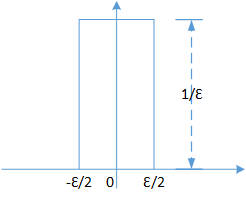
\includegraphics[width=0.4\textwidth]{assets/delta.png}
	\caption{$\delta=\lim\limits_{\epsilon\rightarrow 0}\ \frac{1}{\epsilon}\cdot \Pi_\epsilon(x)$}
\end{figure}
\subsection{脉冲函数的性质}
\begin{enumerate}
	\item $\delta$函数的积分为$1$:
	      $$
		      \int_{-\infty}^{\infty}\ \frac{1}{\epsilon}\cdot \Pi_\epsilon(x)\ dx=\frac{1}{\epsilon}\cdot \int_{-\frac{\epsilon}{2}}^{\frac{\epsilon}{2}}\ 1\ dx=1
	      $$
	\item 如果单单观察$\delta$函数是没有意义的,但是如果$\delta$函数乘上某个函数再积分,就能得到函数在$0$点的值:
	      \begin{align*}
		        & \int_{-\infty}^{\infty}\ \frac{1}{\epsilon}\cdot \Pi_\epsilon(x)\cdot \phi(x)\ dx                                                           \\
		      = & \frac{1}{\epsilon}\cdot \int_{-\frac{\epsilon}{2}}^{\frac{\epsilon}{2}}\ \phi(x)\ dx                                                        \\
		      = & \frac{1}{\epsilon}\cdot \int_{-\frac{\epsilon}{2}}^{\frac{\epsilon}{2}}\ [\phi(0)+\phi'(0)\cdot x+\frac{1}{2}\phi''(0)\cdot x^2+\cdots]\ dx \\
		      = & \phi(0)+o(\epsilon)  = \phi(0)
	      \end{align*}
\end{enumerate}
\subsection{$\delta$的移位}
$$
	\int_{-\infty}^{\infty}\ \delta(a-y)\cdot f(y)\ dy=f(a)
$$
该式子表明了$\delta$从位置$a$处获得函数$f$的值$f(a)$f。我们前面讨论的是$x=0$的情况,在这里,我们定义了一个新的分布,我们记该分布为$\delta_a$。
\subsection{$\delta$的抽样特性}
证明利用到了分布的乘积性质。设有函数$f$:
\begin{align*}
	  & <f\cdot \delta,\phi>                                  \\
	= & <\delta,f\cdot \phi>                                  \\
	= & (f\cdot \phi)(0)   \quad (View\ f(0)\ as\ a\ number.) \\
	= & f(0)\cdot \phi(0)                                     \\
	= & <f(0)\delta,\phi>                                     \\
\end{align*}

因此:
\begin{equation}
	f\cdot \delta=f(0)\cdot \delta
\end{equation}

同理:
\begin{equation}
	f\cdot \delta_a=f(a)\cdot \delta_a
\end{equation}
\subsection{$\delta$的平移特性}
该式子证明利用到了分布的卷积性质。

\subsection{函数$f$与$\delta_a$进行卷积}
\begin{align*}
	  & <f*\delta_a,\phi>                                              \\
	= & <f(x),<\delta_a(y),\phi(x+y)>>                                 \\
	= & <f(x),\phi(x+a)>                                               \\
	= & \int_{-\infty}^{\infty}\ f(u-a)\cdot \phi(u)\ du \quad (u=x+a) \\
	= & <f(u-a),\phi>
\end{align*}

$f$与$\delta_a$进行卷积会导致$f$右移$a$个单位:
\begin{equation}
	f(x)*\delta_a=f(x-a)
\end{equation}

同理可以推导出:
\begin{equation}
	\delta_a*\delta_b=\delta_{a+b}
\end{equation}
\subsection{$\delta$的缩放特性}
该式子证明利用到了分布的卷积性质。

$\delta(x)$是集中于一点的脉冲函数,因此按照我们主观的印象来说,无论怎么在$x$轴对其缩放,都还是原来的脉冲函数,但是事实并不是这样的,我们可以观察下面的推理过程。

当$a>0$时:
\begin{align*}
	  & <\delta(a\cdot x),\phi(x)>                                                                  \\
	= & \int_{-\infty}^{\infty}\ \delta(a\cdot x)\cdot \phi(x)\ dx                                  \\
	= & \int_{-\infty}^{\infty}\ \delta(u)\cdot \phi(\frac{u}{a})\ d(\frac{u}{a})\quad (u=a\cdot x) \\
	= & \frac{1}{a}\cdot \int_{-\infty}^{\infty}\ \delta(u)\cdot \phi(\frac{u}{a})\ du              \\
	= & \frac{1}{a}\cdot<\delta(u),\phi(\frac{u}{a})>                                               \\
	= & \frac{1}{a}\cdot \phi(0)                                                                    \\
	= & <\frac{1}{a}\cdot \delta(x),\phi(x)>
\end{align*}

当$a<0$时:
\begin{align*}
	  & <\delta(a\cdot x),\phi(x)>                                                                  \\
	= & \int_{-\infty}^{\infty}\ \delta(a\cdot x)\cdot \phi(x)\ dx                                  \\
	= & \int_{-\infty}^{\infty}\ \delta(u)\cdot \phi(\frac{u}{a})\ d(\frac{u}{a})\quad (u=a\cdot x) \\
	= & \frac{1}{a}\cdot \int_{\infty}^{-\infty}\ \delta(u)\cdot \phi(\frac{u}{a})\ du              \\
	= & -\frac{1}{a}\cdot<\delta(u),\phi(\frac{u}{a})>                                              \\
	= & -\frac{1}{a}\cdot \phi(0)                                                                   \\
	= & <-\frac{1}{a}\cdot \delta(x),\phi(x)>
\end{align*}

因此:
\begin{equation}
	\delta(a\cdot x)=\frac{1}{|a|}\cdot \delta
\end{equation}
\section{分布}
这里的分布不同于概率上的分布,它是广义函数(generalized function)的另一种说法。
\subsection{测试函数$\phi$}
对于当前研究是最优函数。对于傅立叶变换来说,最优函数就是速降函数。
\subsection{广义函数Generalized Function}
跟这些测试函数相关的,我们称之为广义函数或者分布。

Associated with these test functions is a class of what are called generalized functions of distributions.

一个分布$T$是一个作用于测试函数的线性算子,它作用于测试函数后会产生一个数值,即$T(\phi)$会得到一个数。

A distribution is a linear operation on the test functions that produces a number.

$T$是$\phi$的线性泛函:

The distribution $T$ is a linear functional on test functions.

\begin{align*}
	T(\phi_1+\phi_2)    & =T(\phi_1)+T(\phi_2) \\
	T(\alpha\cdot \phi) & =\alpha\cdot T(\phi)
\end{align*}
\subsection{匹配}
分布作用于$\phi$,我们常称之为匹配,记为$<T,\phi>$:
\begin{equation}
	<T,\phi> = \int_{-\infty}^{\infty}\ T(x)\cdot \phi(x)\ dx
\end{equation}

可以把$\phi$想象成一些物理信息的分布,$T$是一种测量它的方法。使用测量方法去测量一个信息,你将得到一个数。

并非所有函数都会在匹配后积分收敛,但是大多数的函数甚至特别奇异的函数都能使积分收敛,匹配成功。

\subsection{分布的性质}
\begin{enumerate}
	\item 线性
	\item 如果$\phi_n$是一个函数序列收敛于$\phi$,那么如果用$T$作用于$\phi_n$,它也将收敛于$T(\phi)$。
\end{enumerate}



\section{分布傅立叶变换}
\subsection{缓增函数}
在傅立叶变换中,测试函数$\phi$为速降函数。与之对应的分布$T$通常被称为缓增函数(Tempered Distributions):
$$
	<T,\phi>=\int_{-\infty}^{\infty}\ T(x)\cdot \phi(x)\ dx
$$
\subsection{缓增函数的傅立叶变换}
\subsubsection{定义}
定义缓增分布$T$的傅立叶变换为$\mathcal{F}T$,$\mathcal{F}T$作用于速降函数$\phi$就相当于$T$作用于速降函数的傅立叶变换 $\mathcal{F}\phi$:
\begin{equation}
	<\mathcal{F}T,\phi>=<T,\mathcal{F}\phi>
\end{equation}
同理可得,分布的Inverse 傅立叶变换为:
\begin{equation}
	<\mathcal{F}^{-1}T,\phi>=<T,\mathcal{F}^{-1}\phi>
\end{equation}
\subsubsection{证明}
\begin{align*}
	  & <\mathcal{F}T,\phi>                                                                                                     \\
	= & \int_{-\infty}^{\infty}\ \mathcal{F}T(x)\cdot \phi(x)\ dx                                                               \\
	= & \int_{-\infty}^{\infty}\ (\int_{-\infty}^{\infty}\ e^{-2\cdot \pi\cdot i\cdot x\cdot y}\cdot T(y)\ dy)\cdot \phi(x)\ dx \\
	= & \int_{-\infty}^{\infty}\ (\int_{-\infty}^{\infty}\ e^{-2\cdot \pi\cdot i\cdot x\cdot y}\cdot \phi(x)\ dx)\cdot T(y)\ dy \\
	= & \int_{-\infty}^{\infty}\ \mathcal{F}\phi(y)\cdot T(y)\ dy                                                               \\
	= & <T,\mathcal{F}\phi>
\end{align*}

因为$\phi\in \mathcal  {S}$,所以$\mathcal{F}\phi\in \mathcal  {S}$,因此$<T,\mathcal{F}\phi>$是有意义的。至于$<\mathcal{F}T,\phi>$有没有意义,nobody cares。
\subsection{分布傅立叶变换的例子}
\subsubsection{$\mathcal{F}\sigma$}
\begin{align*}
	  & <\mathcal{F}\sigma,\phi>  =  <\sigma,\mathcal{F}\phi>                          \\
	= & \mathcal{F}\phi(0)                                                             \\
	= & \int_{-\infty}^{\infty}\ e^{-2\cdot \pi\cdot i\cdot 0\cdot x}\cdot \phi(x)\ dx \\
	= & \int_{-\infty}^{\infty}\ 1\cdot \phi(x)\ dx                                    \\
	= & <1,\phi>
\end{align*}

因此:
\begin{equation}
	\mathcal{F}\sigma=1
\end{equation}
\begin{figure}[H]
	\centering
	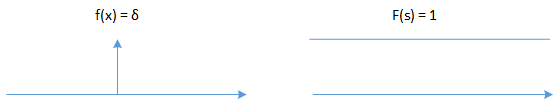
\includegraphics[width=0.4\textwidth]{assets/fdelta.png}
\end{figure}
在$\sigma$的定义中,我们知道$\sigma$无限集中于$0$点,我们通过$\Pi$函数的极限形式来逼近它。而它的傅立叶变换为$1$,这是均匀散开的。还记得我们曾经在讨论傅立叶缩放的时候讲过——时域的集中会导致频域的分散,这就是一个极端的例子。
\subsubsection{$\mathcal{F}\sigma_a$}
\begin{align*}
	  & <\mathcal{F}\sigma_a,\phi>  =  <\sigma_a,\mathcal{F}\phi>                      \\
	= & \mathcal{F}\phi(a)                                                             \\
	= & \int_{-\infty}^{\infty}\ e^{-2\cdot \pi\cdot i\cdot a\cdot x}\cdot \phi(x)\ dx \\
	= & <e^{-2\cdot \pi\cdot i\cdot a\cdot x},\phi>
\end{align*}

因此:
\begin{equation}
	\mathcal{F}\sigma_a=e^{-2\cdot \pi\cdot i\cdot a\cdot x}
\end{equation}

\subsubsection{$\mathcal{F}e^{2\cdot \pi\cdot i\cdot a\cdot x}$}
\begin{align*}
	  & <\mathcal{F}e^{2\cdot \pi\cdot i\cdot a\cdot x},\phi>  =  <e^{2\cdot \pi\cdot i\cdot a\cdot x},\mathcal{F}\phi> \\
	= & \int_{-\infty}^{\infty}\ e^{2\cdot \pi\cdot i\cdot a\cdot x}\cdot \mathcal{F}\phi(x)\ dx                        \\
	= & \mathcal{F}^{-1}\mathcal{F}\phi(a)                                                                              \\
	= & \phi(a)= <\sigma_a,\phi>
\end{align*}

因此:
\begin{equation}
	\mathcal{F}e^{2\cdot \pi\cdot i\cdot a\cdot x}=\sigma_a
\end{equation}
\begin{figure}[H]
	\centering
	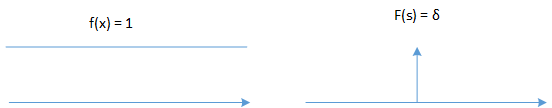
\includegraphics[width=0.4\textwidth]{assets/fe.png}
\end{figure}
当$a=0$时,$e^{2\cdot \pi\cdot i\cdot a\cdot x}=1$,则$\mathcal{F}1=\sigma$。$f(x)=1$的傅立叶变换为$\sigma$,这是一个时域分散导致频域集中的极端例子。
\subsubsection{$\mathcal{F}\cos(2\cdot\pi\cdot a\cdot x)$}
\begin{align*}
	  & \mathcal{F}\cos(2\cdot\pi\cdot a\cdot x)                                                                         \\
	= & \mathcal{F}[\frac{1}{2}\cdot(e^{2\cdot \pi\cdot i\cdot a\cdot x}+e^{-2\cdot \pi\cdot i\cdot a\cdot x})]          \\
	= & \frac{1}{2}\cdot(\mathcal{F}e^{2\cdot \pi\cdot i\cdot a\cdot x}+\mathcal{F}e^{-2\cdot \pi\cdot i\cdot a\cdot x}) \\
	= & \frac{1}{2}\cdot (\sigma_a+\sigma_{-a})
\end{align*}
\begin{figure}[H]
	\centering
	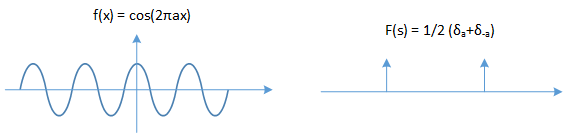
\includegraphics[width=0.4\textwidth]{assets/fcos.png}
\end{figure}
\subsubsection{$\mathcal{F}\sin(2\cdot\pi\cdot a\cdot x)$}
\begin{align*}
	  & \mathcal{F}\sin(2\cdot\pi\cdot a\cdot x)                                                                                \\
	= & \mathcal{F}[\frac{1}{2\cdot i}\cdot(e^{2\cdot \pi\cdot i\cdot a\cdot x}-e^{-2\cdot \pi\cdot i\cdot a\cdot x})]          \\
	= & \frac{1}{2\cdot i}\cdot(\mathcal{F}e^{2\cdot \pi\cdot i\cdot a\cdot x}-\mathcal{F}e^{-2\cdot \pi\cdot i\cdot a\cdot x}) \\
	= & \frac{1}{2\cdot i}\cdot (\sigma_a-\sigma_{-a})
\end{align*}
\begin{figure}[H]
	\centering
	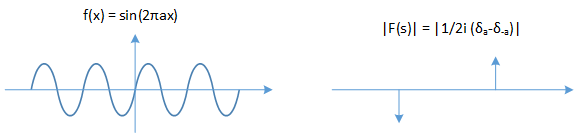
\includegraphics[width=0.4\textwidth]{assets/fsin.png}
\end{figure}
\section{分布与导数}
\subsection{相关定理}
\subsubsection{分布的导数}
\begin{align*}
	  & <T',\phi>                                                                                \\
	= & \int_{-\infty}^{\infty}\ T'(x)\cdot \phi(x)\ dx                                          \\
	= & \rsx{T(x)\cdot \phi(x)}_{-\infty}^\infty-\int_{-\infty}^{\infty}\ T(x)\cdot \phi'(x)\ dx \\
	= & 0-\int_{-\infty}^{\infty}\ T(x)\cdot \phi'(x)\ dx                                        \\
	= & -<T,\phi'>
\end{align*}

所以我们得到:
\begin{equation}
	<T',\phi>=-<T,\phi'>
\end{equation}

由速降函数可知,速降函数的任意阶导都比$x$的任意次幂衰减地都快,即速降函数的任意阶导都是速降函数。因此$\phi'\in \mathcal  {S}$,$<T,\phi'>$仍然成立。
\subsubsection{分布傅立叶变换的导数定理}
分布傅立叶变换的导数定理与傅立叶变换的导数定理类似,注意下面等式中的$s$与$t$:
\begin{equation}
	\mathcal{F}(T')=2\cdot\pi\cdot i\cdot s\cdot \mathcal{F}T
\end{equation}
\begin{equation}
	(\mathcal{F}T)'=\mathcal{F}(-2\cdot\pi\cdot i\cdot t\cdot T)
\end{equation}

\subsection{利用分布求导数的例子}
\subsubsection {单位跃阶函数(Unit Step function)}
\begin{figure}[H]
	\centering
	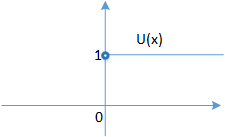
\includegraphics[width=0.4\textwidth]{assets/U_function.png}
	\caption{$\sin(2\cdot\pi\cdot t)+\sin(4\cdot\pi\cdot t)+\sin(8\cdot\pi\cdot t)$}
\end{figure}
\begin{align*}
	U(x)=
	\begin{cases}
		1 & x>0    \\
		0 & x\leq0
	\end{cases}
\end{align*}
下面开始求导:
\begin{align*}
	  & <U',\phi>=-<U(x),\phi'(x)>                                                  \\
	= & -\int_{-\infty}^{\infty}\ U(x)\cdot \phi'(x)\ dx                            \\
	= & -\int_{0}^{\infty}\ \phi'(x)\ dx                                            \\
	= & -\rsx{\phi(x)}_0^\infty                                                     \\
	= & -[0-\phi(0)]   \quad  (\because \lim\limits_{x\rightarrow\pm\inf}\phi(x)=0) \\
	= & \phi(0) = <\delta,\phi>
\end{align*}
因此:
\begin{equation}
	U'=\delta
\end{equation}

由于$U$在原点处有一个跃变,因此它在原点处导数无限大。
\subsubsection {有符号函数(Signum function)}
\begin{figure}[H]
	\centering
	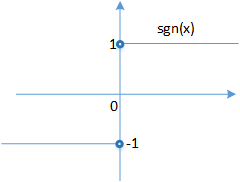
\includegraphics[width=0.4\textwidth]{assets/sgn_function.png}
	\caption{$\sin(2\cdot\pi\cdot t)+\sin(4\cdot\pi\cdot t)+\sin(8\cdot\pi\cdot t)$}
\end{figure}
\begin{align*}
	\sgn(x)=
	\begin{cases}
		1  & x>0 \\
		0  & x=0 \\
		-1 & x<0 \\
	\end{cases}
\end{align*}
下面开始求导:
\begin{align*}
	  & <\sgn',\phi>=<\sgn,\phi'>                                                          \\
	= & -\int_{-\infty}^{\infty}\ \sgn(x)\cdot \phi'(x)\ dx                                \\
	= & -[\int_{-\infty}^{0}\ -1\cdot \phi'(x)\ dx+\int_{0}^{\infty}\ 1\cdot \phi'(x)\ dx] \\
	= & \rsx{\phi(x)}_0^\infty=2\cdot \phi(0)=<2\cdot \sigma,\phi>
\end{align*}
因此:
\begin{equation}
	\sgn'=2\cdot \sigma
\end{equation}

下面求$\sgn$的导数:
\begin{align*}
	  & \mathcal{F}(\sgn)                                             \\
	= & \frac{\mathcal{F}(\sgn')}{2\cdot\pi\cdot i\cdot s}            \\
	= & \frac{2\cdot \delta}{2\cdot\pi\cdot i\cdot s}                 \\
	= & \frac{2}{2\cdot\pi\cdot i\cdot s}=\frac{1}{\pi\cdot i\cdot s} \\
\end{align*}

\subsection{利用导数求傅立叶变换}
\subsubsection {$\sgn$的傅立叶变换}
\begin{align*}
	  & \mathcal{F}(\sgn)                                             \\
	= & \frac{\mathcal{F}(\sgn')}{2\cdot\pi\cdot i\cdot s}            \\
	= & \frac{2\cdot \delta}{2\cdot\pi\cdot i\cdot s}                 \\
	= & \frac{2}{2\cdot\pi\cdot i\cdot s}=\frac{1}{\pi\cdot i\cdot s} \\
\end{align*}
\subsubsection {$U$的傅立叶变换}
\begin{align*}
	U            & =\frac{1}{2}\cdot(1+\sgn)                                                                  \\
	\mathcal{F}U & =\frac{1}{2}\cdot \mathcal{F}(1+\sgn)=\frac{1}{2}\cdot(\sigma+\frac{1}{\pi\cdot i\cdot s})
\end{align*}

在高通滤波器中会用到$U$(单位跃阶)这个信号,采用$U$的傅立叶变换将会加快处理过程。




\section{分布的乘积}
通常情况下被定义为函数与分布的乘积。
设有分布$T$,函数$f$:
\begin{align*}
	  & <T\cdot f,\phi>                                          \\
	= & \int_{-\infty}^{\infty}\ T(x)\cdot f(x)\cdot \phi(x)\ dx \\
	= & <T,f\cdot \phi>
\end{align*}
\section{分布与卷积}
\subsection{分布的卷积}
假设有函数$f$与速降函数$\psi$,他们的卷积为$f*\psi$:
\begin{align*}
	  & <\psi*f,\phi>                                                                                  \\
	= & \int_{-\infty}^{\infty}\ (\psi*f)(x)\cdot \phi(x)\ dx                                          \\
	= & \int_{-\infty}^{\infty}\ [\int_{-\infty}^{\infty}\ \psi(x-y)\cdot f(y)\ dy]\cdot \phi(x)\ dx   \\
	= & \int_{-\infty}^{\infty}\ [\int_{-\infty}^{\infty}\ \psi(x-y)\cdot \phi(x)\ dx]\cdot f(y)\ dy   \\
	= & \int_{-\infty}^{\infty}\ [\int_{-\infty}^{\infty}\ \psi^-(y-x)\cdot \phi(x)\ dx]\cdot f(y)\ dy \\
	= & \int_{-\infty}^{\infty}\ (\psi^-*\phi)(y)\cdot f(y)\ dy                                        \\
	= & <f,\psi^-*\phi>
\end{align*}

进一步推导:
\begin{align*}
	  & \psi^-*\phi                                                       \\
	= & \int_{-\infty}^{\infty}\ \psi(x-y)\cdot \phi(x)\ dx               \\
	= & \int_{-\infty}^{\infty}\ \psi(u)\cdot \phi(u+y)\ du \quad (u=x-y) \\
	= & <\psi(u),\phi(u+y)>
\end{align*}

把推导结果代入卷积的推导中,得:
$$
	<\psi*f,\phi>=<f(x),<\psi(y),\phi(x+y)>>
$$

推广到一般的分布中去,设有分布$S$和$T$:
\begin{equation}
	<S*T,\phi>=<S(x),<T(y),\phi(x+y)>>
\end{equation}

分布卷积成立的条件如下:

$<T(y),\phi(x+y)>$将产生一个变量为$x$的函数,只有当该函数为测试函数时,$S*T$才有意义。
\subsection{分布的卷积定理}
我们在分析传统傅立叶变换的卷积定理的时候,是结合卷积与傅立叶变换一起讨论的。在分布中,通常也会把卷积与傅立叶变换一起讨论。
\begin{align*}
	  & <\mathcal{F}(S*T),\phi>                     \\
	= & <S*T,\mathcal{F}\phi>                       \\
	= & <S,T^-*\mathcal{F}\phi>                     \\
	= & <S,\mathcal{F}\mathcal{F}T*\mathcal{F}\phi> \\
	= & <S,\mathcal{F}(\mathcal{F}T\cdot \phi)>     \\
	= & <\mathcal{F}S,\mathcal{F}T\cdot \phi>       \\
	= & <\mathcal{F}S\cdot \mathcal{F}T,\phi>
\end{align*}

因此:
\begin{equation}
	\mathcal{F}(S*T)=\mathcal{F}S\cdot \mathcal{F}T
\end{equation}
该定理成立的条件与卷积成立的条件一致,即$T^−$与速降函数进行卷积后仍然是速降函数。

采样定理于1928年由美国物理学家H.奈奎斯特首先提出来,因此被称为奈奎斯特采样定理。1933年,苏联工程师科捷利尼科夫首次用公式严格地表述了这一定理,因此在苏联的文献中称其为科捷利尼科夫采样定理。1948年,信息论的创始人C·E·香农对这一定理加以明确的说明,并正式作为定理引用,因此在许多文献中又称为香衣采样定理。